\documentclass[14pt]{article}

\usepackage{amsmath}
\usepackage{graphicx}
\usepackage{hyperref}

\title{de Bruijn project}
\author{Sergey Nurk, Anton Bankevich and Nikolay Vyahhi}
\date{\today}

\begin{document}

\maketitle

\section{Common Classes}

We have two classes for Sequences (all use 2 bits per nucleotide) in \texttt{src/common/}:
\begin{itemize}
\item \texttt{Seq$<$size\_t size$>$} -- immutable ACGT-sequence with compile-time length (= template argument \texttt{size}) and zero memory overhead.
\item \texttt{Sequence} --- immutable ACGT-sequence with run-time length and some constant memory overhead. It stores sequence in helper class \texttt{SequenceData} with reference counting. Usually both straight and reverse-complement sequence share the same \texttt{SequenceData} object. Substring is O(1) operation for \texttt{Sequence}.
\end{itemize}

\section{Graph Construction}

First we construct usual de Bruijn node-graph with:
\begin{itemize}
\item K-mers as nodes,
\item (K+1)-mers as edges.
\end{itemize}
for some compile-time fixed K. 

\textit{Comment: Yes, it'll be better to make it runtime-length later.} \\

It's \texttt{DeBruijn<int size>} class in \texttt{src/debruijn/debruijn.hpp}, where \texttt{size} is length of K-mer (i.e. \texttt{size} = K). \\

In practice, \texttt{DeBruijn} class stores only nodes with information about incoming and outgoing edges --- map from K-mer to some \texttt{DeBruijn::Data}. Now it's \texttt{std::tr1::unordered\_map} (standard C++0x hashmap), later it'll probably be replaced with Cuckoo hashmap (now in \texttt{src/common/cuckoo.hpp}). Cuckoo have higher load factor (90-95\%, hence very memory-effective), much slower \texttt{insert} but much faster \texttt{find}.

\begin{itemize}
\item K-mer as \texttt{Seq$<$size$>$}.
\item \texttt{DeBruijn::Data} stores 8 \texttt{size\_t} counters for $4$ incoming and $4$ outgoing edges.

\textit{Comment \#1: Since we don't need coverage here, we can reduce memory to only $1$ byte ($4+4$ bits) instead of $8*4=32$ bytes for counters.}
 
\textit{Comment \#2: Even if we need counters, we can mostly use \texttt{char} instead of \texttt{size\_t} here.}
\end{itemize}

\section{Graph Simplification / Condensing}

We observed that it's more effective to construct new (condensed) graph from \texttt{DeBruijn} graph than to try to condense \texttt{DeBruijn} itself. So new \texttt{edge\_graph::EdgeGraph} (\texttt{src/debruijn/edge\_graph.hpp} is constructed from \texttt{DeBruijn} graph. It's done by usual traversal and accumulating edge-sequence while we're on a simple path (path without branchings). \\

Every \texttt{edge\_graph::Edge} stores:
\begin{itemize}
\item it's \texttt{Sequence},
\item end \texttt{Vertex},
\item \texttt{size\_t} coverage -- how much times (K+1)-mers from this edge was observed in original reads. It's additive, so we can simply join two edges and sum their coverages. This coverage will be filled during Read Threading (below).
\end{itemize} \vspace{.5 cm}

Every \texttt{edge\_graph::Vertex} stores:
\begin{itemize}
\item \texttt{vector$<$Edge*$>$} of outgoing edges.
\item \texttt{Vertex*} -- reverse-complement \texttt{Vertex}.
\end{itemize} \vspace{.5 cm}

Also old \texttt{DeBruijn} graph isn't waste of memory. From now it acts as the index for new \texttt{EdgeGraph}. It maps K-mers to edges which contains this K-mer. \textit{Comment: Is it already implemented or only in plans?}
 
\section{Sequences (Reads) Mapping}

After graph construction and simplification all original reads are mapped to the edges (path) of resulting \texttt{EdgeGraph} using \texttt{SimpleSequenceMaper::MapSequence()} (\texttt{src/debruijn/utils.hpp}). By that we calculate \texttt{Edge::coverage} for all edges in \texttt{EdgeGraph}.

\textit{Comment: Now this function uses \texttt{SimpleIndex} from \texttt{utils.hpp}, but it can be substituted by \texttt{DeBruijn} later.} 

\section{Smart Iterators}

\texttt{EdgeGraph} have 2 types of smart iterators (\texttt{src/debruijn/utils.hpp}):
\begin{itemize}
\item \texttt{SmartEdgeIterator$<$Graph, Comparator$>$} -- to iterate over all edges.
\item \texttt{SmartVertexIterator$<$Graph, Comparator$>$} -- to iterate over all vertices.
\end{itemize}
They are used for all graph operation below (e.g. tips clipping and bulges removal). \\

Comparator is a less-functor (class with \texttt{operator()}) for edges/vertices. It compares two objects $e_1$ and $e_2$ and returns true iff $e_1 < e_2$. E.g. \texttt{std::less<EdgeId>}. \\

This iterators are smart not because they have such class-name, but because edges/vertices insert/delete operators don't invalidate them. Hence this iterators can be used to traverse the graph while dynamically change it (e.g. for tips clipping and bulges removal). \\

Smart iterators are template-classes, so they work with any \texttt{Graph} that supports some operations (\textit{TODO: write which ones!}) and with any \texttt{Comparator} (\texttt{less} for edges/vertices for ordering traversal, e.g. from lower coverage to higher). \\

This iterators use standard \texttt{std::set} to store, order and update edges/vertices which should be traversed. It requires additional ammount of memory equal to $O(\#edges)$/$O(\#vertices)$. But since \texttt{Sequence}s are major memory-consumers, this overhead is not sufficient.

\section{Tips Clipping (TC)}

Using \texttt{SmartEdgeIterator} we traverse graph from smaller edge-length to bigger (\texttt{src/debruijn/tip\_clipper.hpp}). We delete edge (tip) from the graph iff:
\begin{itemize}
\item It's end-vertex have no outgoing edges. We can skip check of start-vertex here since we traverse both straight edge and it's reverse-complementary edge during TC. 
\item It has length $<$ \texttt{DEFAULT\_MAX\_TIP\_LENGTH} (50 now).
\item It has coverage $<$ \texttt{DEFAULT\_COVERAGE\_BOUND} (1000 now, like infinity).
\item It has relative coverage $<$ \texttt{DEFAULT\_RELATIVE\_COVERAGE\_BOUND} (2.0 now). It means that tip's coverage is at most \texttt{DEFAULT\_RELATIVE\_COVERAGE\_BOUND} times (max coverage over all edges outgoing from the same vertex).
\end{itemize} \vspace{0.5 cm}

To delete tip we ask graph to delete this edge. Default graph implementation additionally deletes its end-vertex and its reverse-complementary edge. \\

We condense (join) new simple path after the tip was clipped only iff:
\begin{itemize}
\item There is only one more edge outgoing from the start-vertex of removed tip.
\item This only edge is also a tip.
\end{itemize}
It's required for proper clipping of this another tip. \\

Any other case of condensing is not necessary to be handled on-line during the TC (and even can lead to quadratic complexity in worst case because of too much \texttt{Sequence} joins). So we condense any other simple pathes only after all tips were clipped. \\

\textit{Comment: Now all parameters are \texttt{\#define}s, but it's better to make them tunable.}

\section{Bulges Removal (BR)}

Method \texttt{BulgeRemover::RemoveBulges()} (from \texttt{src/debruijn/bulge\_remover.hpp}) walks through the graph and removes bulges. The bulge is edge (not path!) with:
\begin{itemize}
\item Difference between this edge's length and the length of other alternative path (between it's start-vertex and end-vertex) is less then $\delta$. Now $\delta = 3$ (hardcoded. oh... should be as parameter).
\item Coverage less then $1.1$ * (alternative path's coverage). (hardcoded value too).
\item Coverage less then some fixed coverage \textit{(TODO: isn't in code now)}.
\end{itemize} \vspace{0.5 cm}

\textit{Comment: define alternative path.} \\

After every bulge removal all new simple pathes are condensed (they can be formed only near start-vertex and end-vertex, not deeply inside alternative path). \\

\textit{TODO: Transfer coverage from bulge to alternative path.}

\textit{TODO: Transfer edge-pair distance from bulge to alternative path.}

\section{Mate Pairs (Edge-Pairs) Distance}

\textit{TODO: Handle it, not implemented now.}

\section{Evaluation}

All Quake-filtered reads were cropped to first $100$ kilo-basepairs of E.Coli. I.e. we try to assemble only first $100$kbp of E.Coli (for simplicity). Also, for evaluation runs we use only 1st read from every mate pair. It's total of $306174$ error-corrected reads with $100$ or less basepairs each.

\subsection{Log 100k}
(first column is milliseconds from the starting time, $\approx 5.6$ minutes total): \\

\noindent\scriptsize{\texttt{310  INFO d.edge\_graph (edge\_graph\_tool.hpp:95) - Edge graph construction tool started \\
    311  INFO d.edge\_graph (edge\_graph\_tool.hpp:53) - Constructing DeBruijn graph \\
  14928  INFO d.edge\_graph (edge\_graph\_tool.hpp:55) - DeBruijn graph constructed \\
  14928  INFO d.edge\_graph (edge\_graph\_tool.hpp:61) - Condensing graph \\
  23146  INFO d.edge\_graph (edge\_graph\_tool.hpp:64) - Graph condensed \\
  23146  INFO d.edge\_graph (edge\_graph\_tool.hpp:66) - Counting coverage \\
  32289  INFO d.edge\_graph (edge\_graph\_tool.hpp:69) - Coverage counted \\
  32289  INFO d.edge\_graph (edge\_graph\_tool.hpp:22) - Counting stats \\
  32289  INFO d.edge\_graph (edge\_graph\_tool.hpp:27) - Vertex count=790; Edge count=836 \\
  32289  INFO d.edge\_graph (edge\_graph\_tool.hpp:28) - Stats counted \\
  32319  INFO d.edge\_graph (edge\_graph\_tool.hpp:34) - Writing graph 'edge\_graph' to file edge\_graph.dot \\
  32911  INFO d.edge\_graph (edge\_graph\_tool.hpp:36) - Graphraph 'edge\_graph' written to file edge\_graph.dot \\
  32911  INFO d.edge\_graph (edge\_graph\_tool.hpp:75) - Clipping tips \\
  33114  INFO d.edge\_graph (edge\_graph\_tool.hpp:79) - Tips clipped \\
  33114  INFO d.edge\_graph (edge\_graph\_tool.hpp:22) - Counting stats \\
  33114  INFO d.edge\_graph (edge\_graph\_tool.hpp:27) - Vertex count=118; Edge count=164 \\
  33114  INFO d.edge\_graph (edge\_graph\_tool.hpp:28) - Stats counted \\
  33146  INFO d.edge\_graph (edge\_graph\_tool.hpp:34) - Writing graph 'no\_tip\_graph' to file tips\_clipped.dot \\
  33180  INFO d.edge\_graph (edge\_graph\_tool.hpp:36) - Graphraph 'no\_tip\_graph' written to file tips\_clipped.dot \\
  33180  INFO d.edge\_graph (edge\_graph\_tool.hpp:85) - Removing bulges \\
  33563  INFO d.edge\_graph (edge\_graph\_tool.hpp:88) - Bulges removed \\
  33563  INFO d.edge\_graph (edge\_graph\_tool.hpp:22) - Counting stats \\
  33563  INFO d.edge\_graph (edge\_graph\_tool.hpp:27) - Vertex count=70; Edge count=92 \\
  33563  INFO d.edge\_graph (edge\_graph\_tool.hpp:28) - Stats counted \\
  33598  INFO d.edge\_graph (edge\_graph\_tool.hpp:34) - Writing graph 'no\_bulge\_graph' to file bulges\_removed.dot \\
  33602  INFO d.edge\_graph (edge\_graph\_tool.hpp:36) - Graphraph 'no\_bulge\_graph' written to file bulges\_removed.dot \\
  33602  INFO d.edge\_graph (edge\_graph\_tool.hpp:115) - Tool finished \\
}}

\newpage
\begin{figure}
\begin{center}
\includegraphics[width=0.7\textwidth]{edge_graph.pdf}
\end{center}
\caption{Edge Graph 100k (790 vertices, 836 edges)}
\end{figure}

\newpage

\begin{figure}
\begin{center}
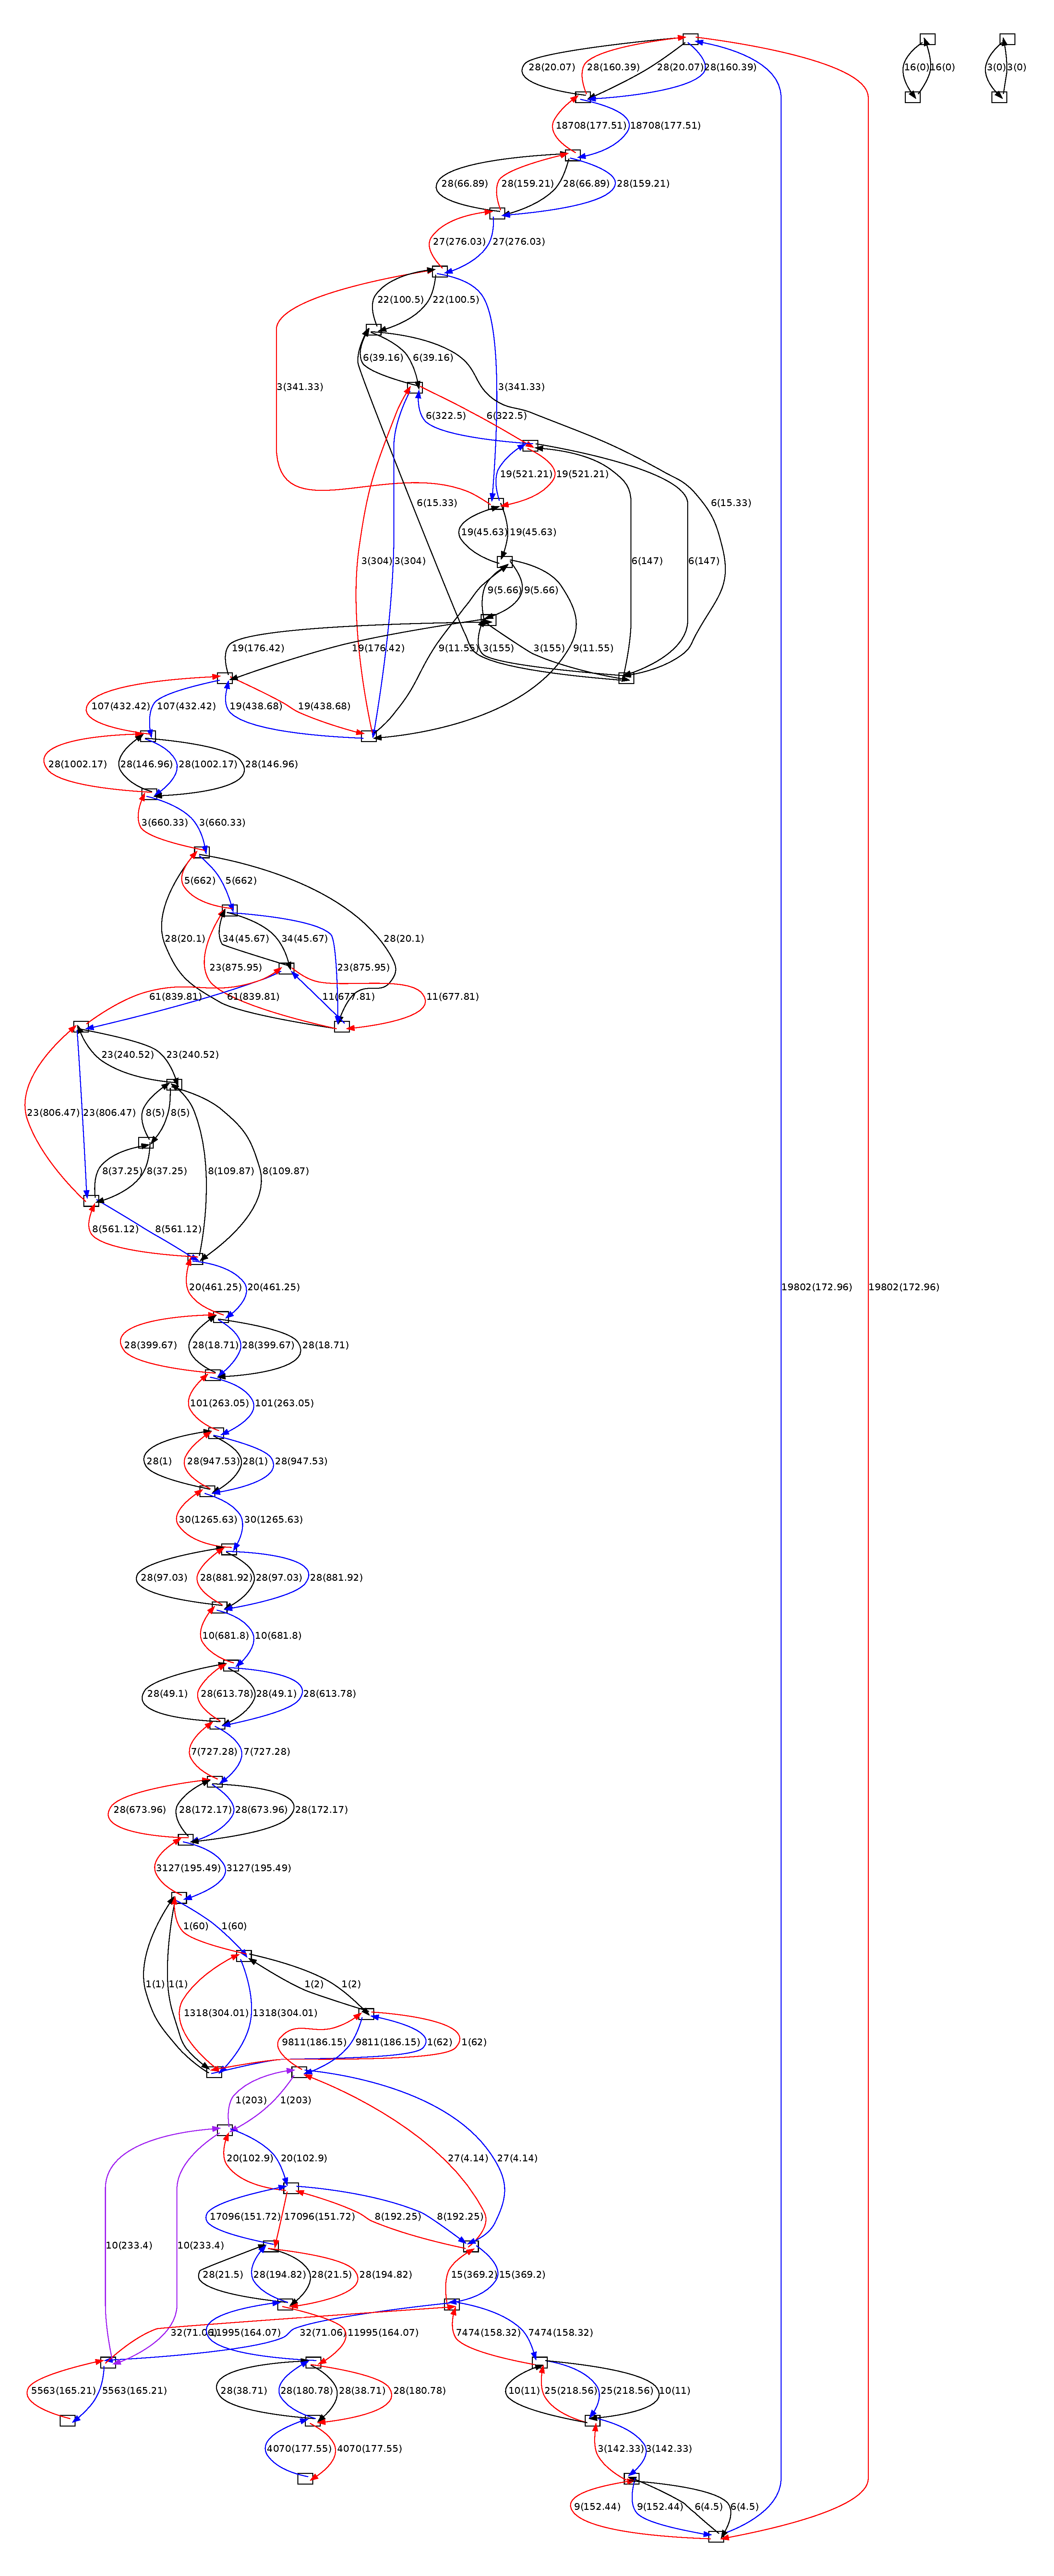
\includegraphics[width=0.7\textwidth]{tips_clipped.pdf}
\end{center}
\caption{Edge Graph 100k after TC (118 vertices, 164 edges)}
\end{figure}

\newpage

\begin{figure}
\begin{center}
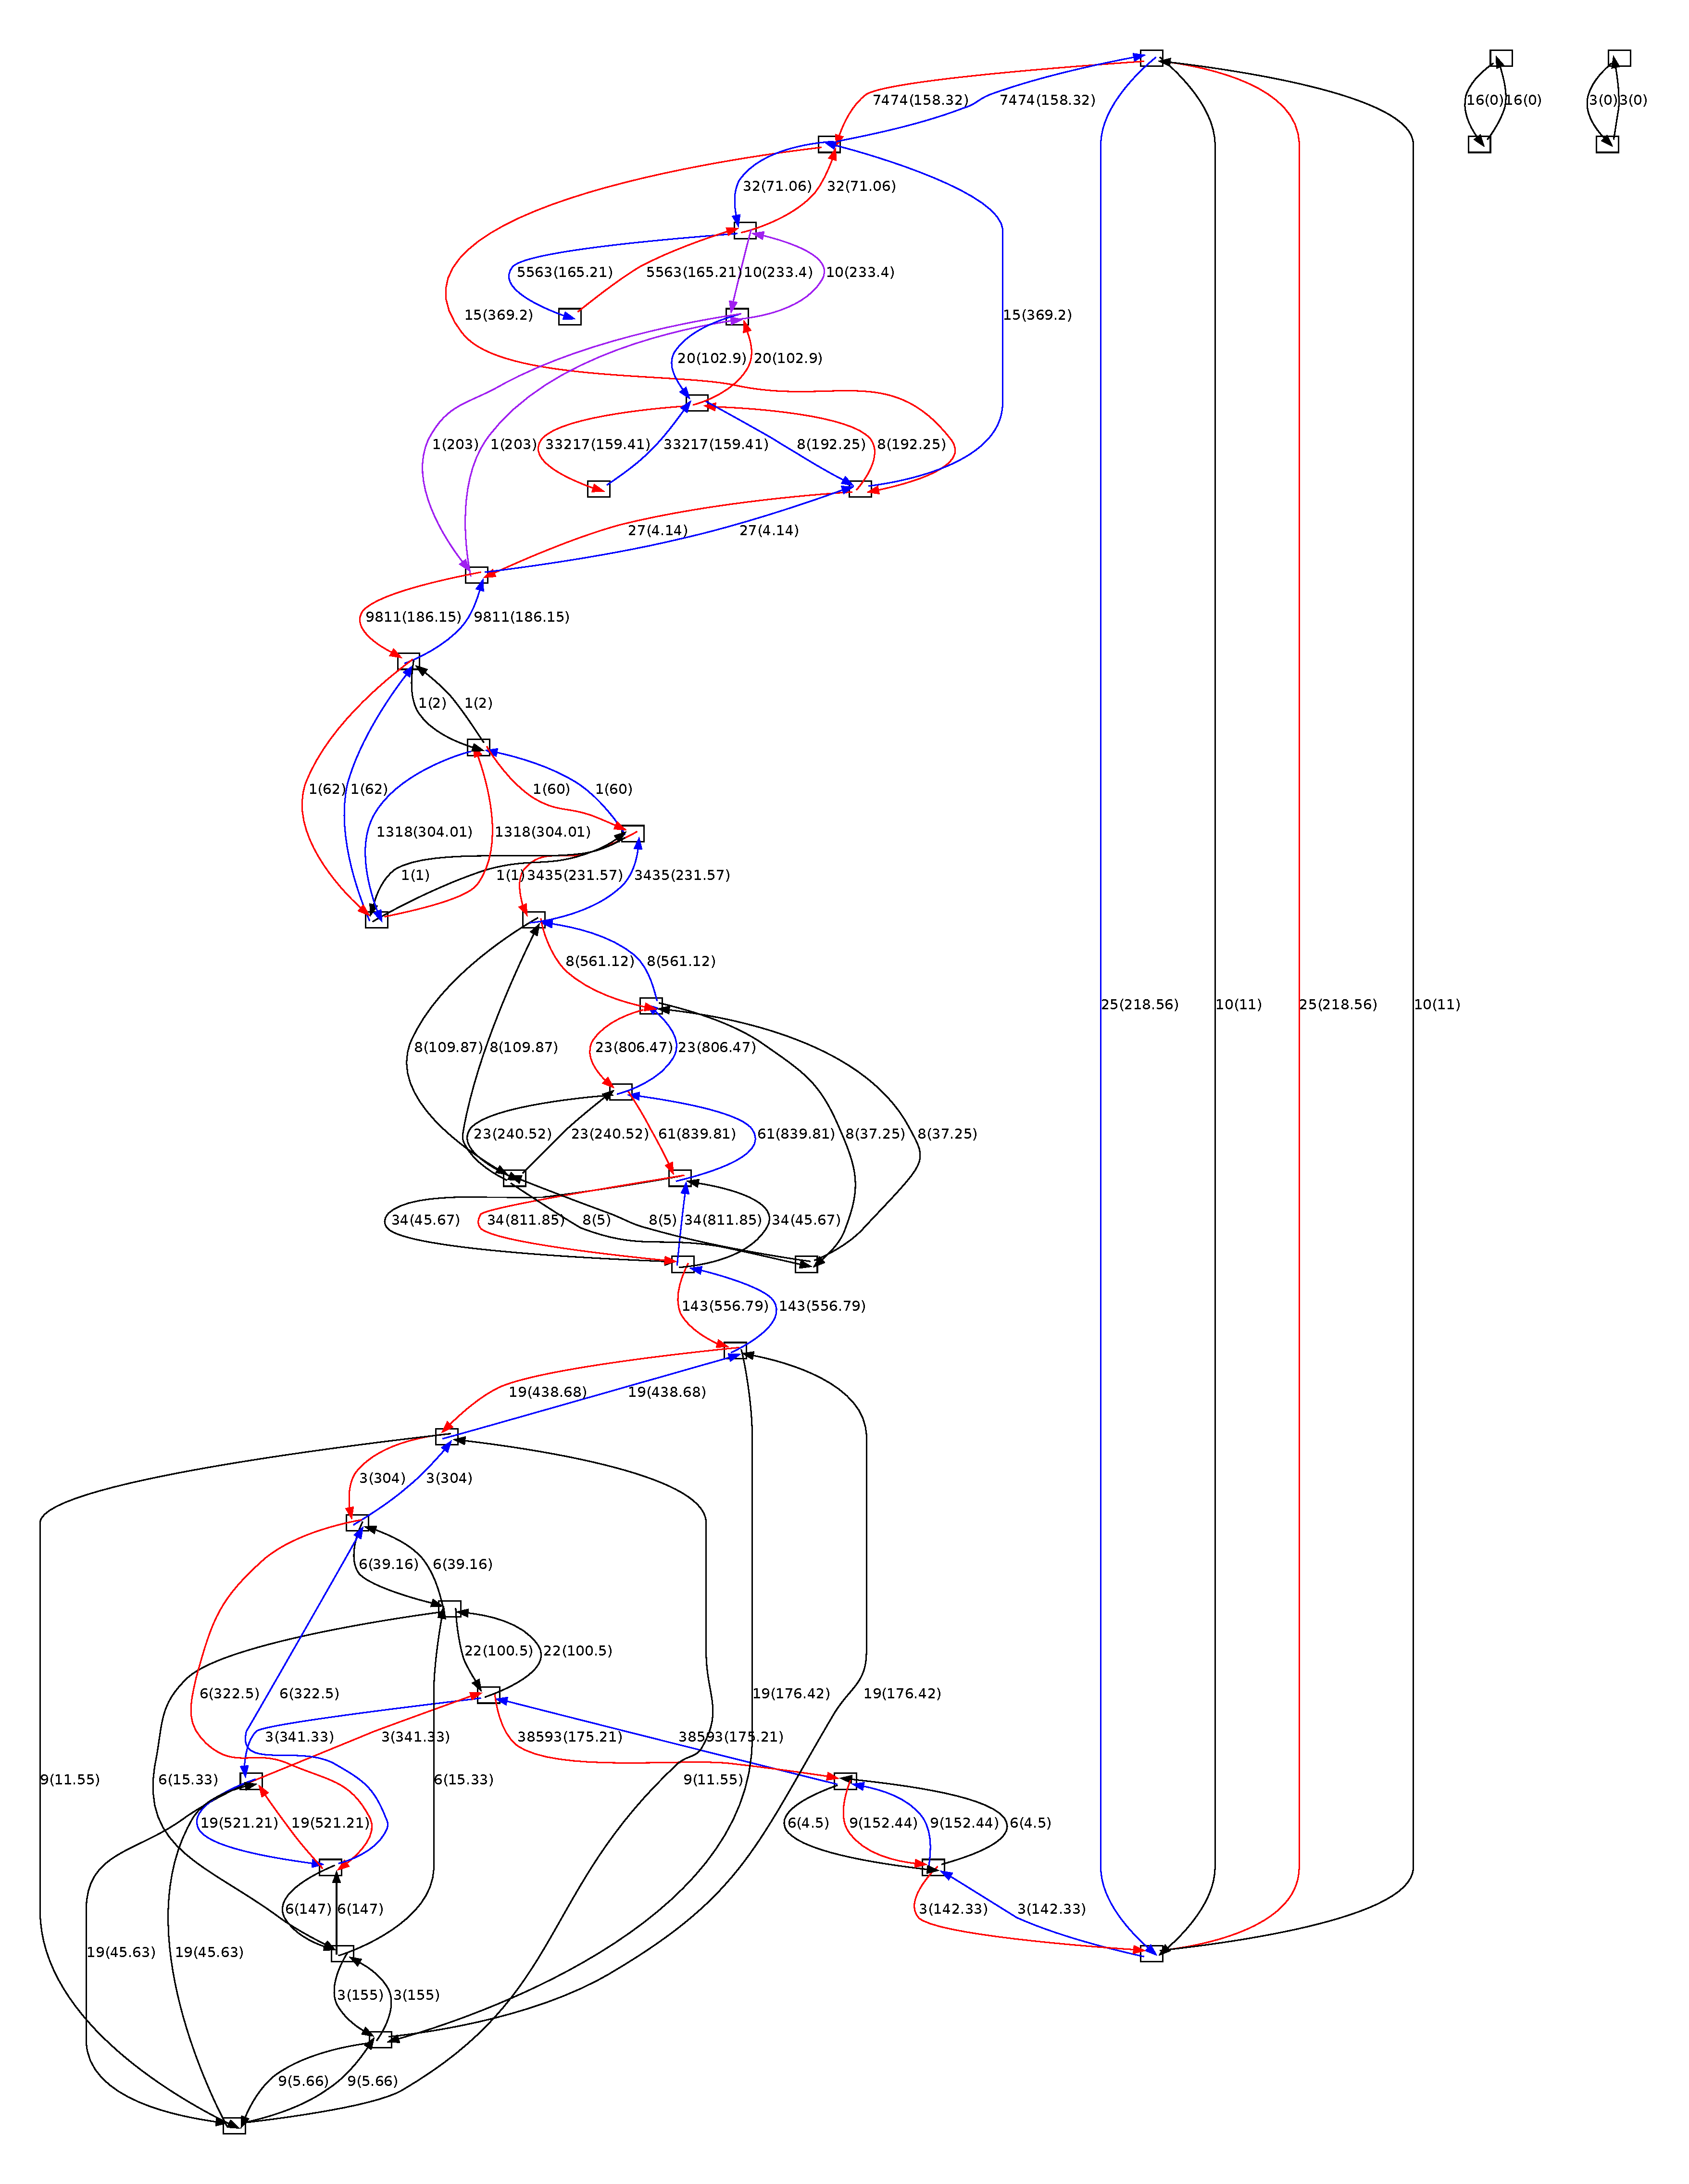
\includegraphics[width=0.7\textwidth]{bulges_removed.pdf}
\end{center}
\caption{Edge Graph 100k after TC+BR (70 vertices, 92 edges)}
\end{figure}

\end{document}